\documentclass[aspectratio=169,11pt]{beamer}

\usepackage[utf8]{inputenc}
\usepackage[T1]{fontenc}
\usepackage[english]{babel}
\usepackage{amsmath,amssymb}
\usepackage{booktabs}
\usepackage{graphicx}
\usepackage{listings}
\usepackage{xcolor}

\usetheme{default}
\usecolortheme{seahorse}

\setbeamertemplate{navigation symbols}{}
\setbeamertemplate{footline}[frame number]
\setbeamerfont{frametitle}{size=\large}
\setbeamerfont{title}{size=\Large}
\setbeamerfont{subtitle}{size=\normalsize}

\lstdefinelanguage{Lean}{
  morekeywords={theorem,def,by,intro,exact,constructor,Prop},
  sensitive=true,
  morecomment=[l]{--},
  morestring=[b]"
}

\lstset{
  language=Lean,
  basicstyle=\ttfamily\scriptsize,
  columns=fullflexible,
  breaklines=true,
  showstringspaces=false,
  literate=
    {ℝ}{{$\mathbb{R}$}}1
    {⟨}{{$\langle$}}1
    {⟩}{{$\rangle$}}1
}

\title{Acemoglu \& Restrepo (2018)}
\subtitle{\emph{The Race between Man and Machine}}
\author{Carlos Gómez Puican}
\date{Repository 6 \textperiodcentered{} September 2026}

\begin{document}

% ============================================================
% TITLE
% ============================================================

\begin{frame}[plain]
  \titlepage

  \begin{center}
    \small
    \texttt{github.com/carlosgomezp28/ai-06-restrepo}
  \end{center}
\end{frame}

% ============================================================
% 1
% ============================================================

\begin{frame}{1 \textperiodcentered{} Question and unit of analysis}

  \textbf{Question.}
  How do automation and the creation of new tasks affect output,
  wages, employment, and factor shares?

  \medskip

  \textbf{Key shift relative to the other papers.}

  \begin{itemize}\small
    \item The unit of analysis is the \textbf{aggregate economy},
    not an individual worker or AI agent.

    \item Technology changes \emph{which tasks} capital and labor perform.

    \item The central race is between
    \textbf{displacement} and \textbf{reinstatement}.
  \end{itemize}

  \medskip

  \textbf{Static environment.} A unit measure of tasks is indexed by

  \[
    i\in[N-1,N].
  \]

\end{frame}

% ============================================================
% 2
% ============================================================

\begin{frame}{2 \textperiodcentered{} The firm's task-level problem}

  Labor productivity in task $i$ is $\gamma(i)$, with
  $\gamma(i)$ strictly increasing.

  \medskip

  If task $i$ is technologically automatable, the firm compares

  \[
    R
    \qquad\text{vs.}\qquad
    \frac{W}{\gamma(i)}.
  \]

  \begin{itemize}\small
    \item $R$: rental rate of capital.
    \item $W/\gamma(i)$: effective unit cost of labor in task $i$.
    \item Higher-index tasks are those in which labor has stronger
    comparative advantage.
  \end{itemize}

  \medskip

  \textbf{Agent's problem:}
  competitive firms assign each task to the lowest-cost feasible factor.

\end{frame}

% ============================================================
% 3
% ============================================================

\begin{frame}{3 \textperiodcentered{} Technology and the equilibrium cutoff}

  Automation technology is summarized by $I\in[N-1,N]$:

  \[
    i\le I
    \Rightarrow
    \text{capital is technologically feasible},
  \]

  \[
    i>I
    \Rightarrow
    \text{labor only}.
  \]

  The cost-indifference threshold $\widetilde I$ solves

  \[
    \frac{W}{R}=\gamma(\widetilde I).
  \]

  Therefore equilibrium automation is

  \[
    \boxed{I^*=\min\{I,\widetilde I\}}.
  \]

  \begin{center}
    \small
    $i\le I^*$: capital
    \qquad\qquad
    $i>I^*$: labor
  \end{center}

\end{frame}

% ============================================================
% 4
% ============================================================

\begin{frame}{4 \textperiodcentered{} Conditions behind the static results}

  The main static propositions impose Assumptions 1--3.

  \begin{enumerate}\small

    \item $\gamma(i)$ is strictly increasing.

    \item Either
    \[
      \eta\to0
      \qquad\text{or}\qquad
      \zeta=1.
    \]
    This delivers homothetic factor demands in the baseline exposition.

    \item $K<\overline K$, where $\overline K$ is defined by
    \[
      R=\frac{W}{\gamma(N)}.
    \]

  \end{enumerate}

  Hence in the maintained region

  \[
    R>\frac{W}{\gamma(N)},
  \]

  so newly created tasks are profitable to use immediately.

  \medskip

  Under these conditions the static equilibrium exists and is unique.

\end{frame}

% ============================================================
% 5
% ============================================================

\begin{frame}{5 \textperiodcentered{} Proposition 2: technology-constrained automation}

  Consider

  \[
    I^*=I<\widetilde I.
  \]

  The range of automated tasks is constrained by available technology.

  For automation,

  \[
    \frac{d\ln(W/R)}{dI}
    =
    -\frac{\Lambda_I}
    {\widehat\sigma+\varepsilon_L}
    <0.
  \]

  \begin{block}{Sign implications}
    A rise in $I$ reduces $W/R$, the labor share, and employment.
  \end{block}

  The sign of the \textbf{real wage} $W$ is not pinned down by
  this result alone.

\end{frame}

% ============================================================
% 6
% ============================================================

\begin{frame}{6 \textperiodcentered{} When more automation technology does nothing}

  Now consider

  \[
    I^*=\widetilde I<I.
  \]

  Firms are already choosing the cost-minimizing boundary.

  \medskip

  More technically automatable tasks do not change the allocation
  at the margin.

  \medskip

  Therefore a marginal increase in $I$ has no effect on
  equilibrium factor prices.

  \medskip

  \begin{center}
    \boxed{
      \text{Technological feasibility }I
      \neq
      \text{ equilibrium automation }I^*
    }
  \end{center}

\end{frame}

% ============================================================
% 7
% ============================================================

\begin{frame}{7 \textperiodcentered{} The two forces}

  \begin{columns}[T]

    \column{0.48\textwidth}

    \textbf{Automation: displacement}

    \begin{itemize}\small
      \item Expands tasks performed by capital.
      \item Contracts the task range performed by labor.
      \item Pushes relative labor demand downward.
    \end{itemize}

    \column{0.48\textwidth}

    \textbf{New tasks: reinstatement}

    \begin{itemize}\small
      \item Raises $N$.
      \item Introduces tasks where labor has comparative advantage.
      \item Raises relative labor demand.
    \end{itemize}

  \end{columns}

  \medskip

  \begin{center}
    The long-run model is a race between these two margins.
  \end{center}

\end{frame}

% ============================================================
% 8
% ============================================================

\begin{frame}{8 \textperiodcentered{} Proposition 3: the wage decomposition}

  Under Assumptions 1--3, in the technology-constrained regime,

  \[
  \begin{aligned}
  d\ln W
  ={}&
  d\ln Y\big|_{K,L}
  \\
  &+
  (1-s_L)
  \left[
    \frac{\Lambda_N}
    {\widehat\sigma+\varepsilon_L}dN
    -
    \frac{\Lambda_I}
    {\widehat\sigma+\varepsilon_L}dI
  \right].
  \end{aligned}
  \]

  For a pure automation shock, $dN=0$ and $dI>0$:

  \[
    d\ln W
    =
    \underbrace{
      d\ln Y\big|_{K,L}
    }_{\text{productivity }(+)}
    -
    \underbrace{
      (1-s_L)
      \frac{\Lambda_I}
      {\widehat\sigma+\varepsilon_L}dI
    }_{\text{displacement }(-)}.
  \]

\end{frame}

% ============================================================
% 9
% ============================================================

\begin{frame}{9 \textperiodcentered{} The week's trap: does automation necessarily lower wages?}

  \textbf{No.}

  \medskip

  Automation in the technology-constrained regime always lowers
  $W/R$, but

  \[
    \boxed{
    dW>0
    \iff
    \text{productivity effect}
    >
    \text{displacement effect}
    }.
  \]

  \begin{itemize}\small

    \item \textbf{Productivity:}
    replacing expensive labor with cheaper capital raises output
    holding $K,L$ fixed.

    \item \textbf{Displacement:}
    labor is squeezed into a smaller set of tasks.

  \end{itemize}

  \medskip

  So $W\uparrow$ can coexist with

  \[
    \text{labor share}\downarrow,
    \qquad
    \text{employment}\downarrow.
  \]

\end{frame}

% ============================================================
% 10
% ============================================================

\begin{frame}{10 \textperiodcentered{} Proposition 3: the capital-stock threshold}

  Still under Assumptions 1--3 and

  \[
    I^*=I<\widetilde I,
  \]

  Proposition 3 implies that there exists a finite threshold
  $\widetilde K$ such that

  \[
    K>\widetilde K
    \quad\Longrightarrow\quad
    \frac{dW}{dI}>0,
  \]

  while

  \[
    K<\widetilde K
    \quad\Longrightarrow\quad
    \frac{dW}{dI}<0.
  \]

  \medskip

  \textbf{Interpretation.}
  A larger capital stock makes the cost-saving/productivity channel
  from automation strong enough to dominate displacement.

\end{frame}

% ============================================================
% 11
% ============================================================

\begin{frame}{11 \textperiodcentered{} What I did}

  \begin{itemize}\small

    \item Reconstructed the task-allocation logic:
    $I$, $\widetilde I$, and $I^*$.

    \item Re-derived by hand why
    \[
      \frac{d\ln(W/R)}{dI}<0
    \]
    does \emph{not} imply
    \[
      \frac{dW}{dI}<0.
    \]

    \item Checked the productivity-versus-displacement condition
    and the $\widetilde K$ threshold.

    \item Ran my own AppliedModelingLib formalization as
    \texttt{AR18RaceManMachine}.

    \item Repaired three proof/build issues without changing
    statements or economic assumptions.

    \item Final paper-scoped check:
    \texttt{832 jobs}, exit code \texttt{0}.

  \end{itemize}

  \medskip

  \textbf{Computational contribution:}
  formal verification of selected reduced-form comparative-statics
  claims, with an auditable build/check trail.

\end{frame}

% ============================================================
% 12
% ============================================================

\begin{frame}{12 \textperiodcentered{} Where I did not believe the AI: hand check I}

  \centering

  \IfFileExists{hand/prop3-automation-wages.pdf}{
    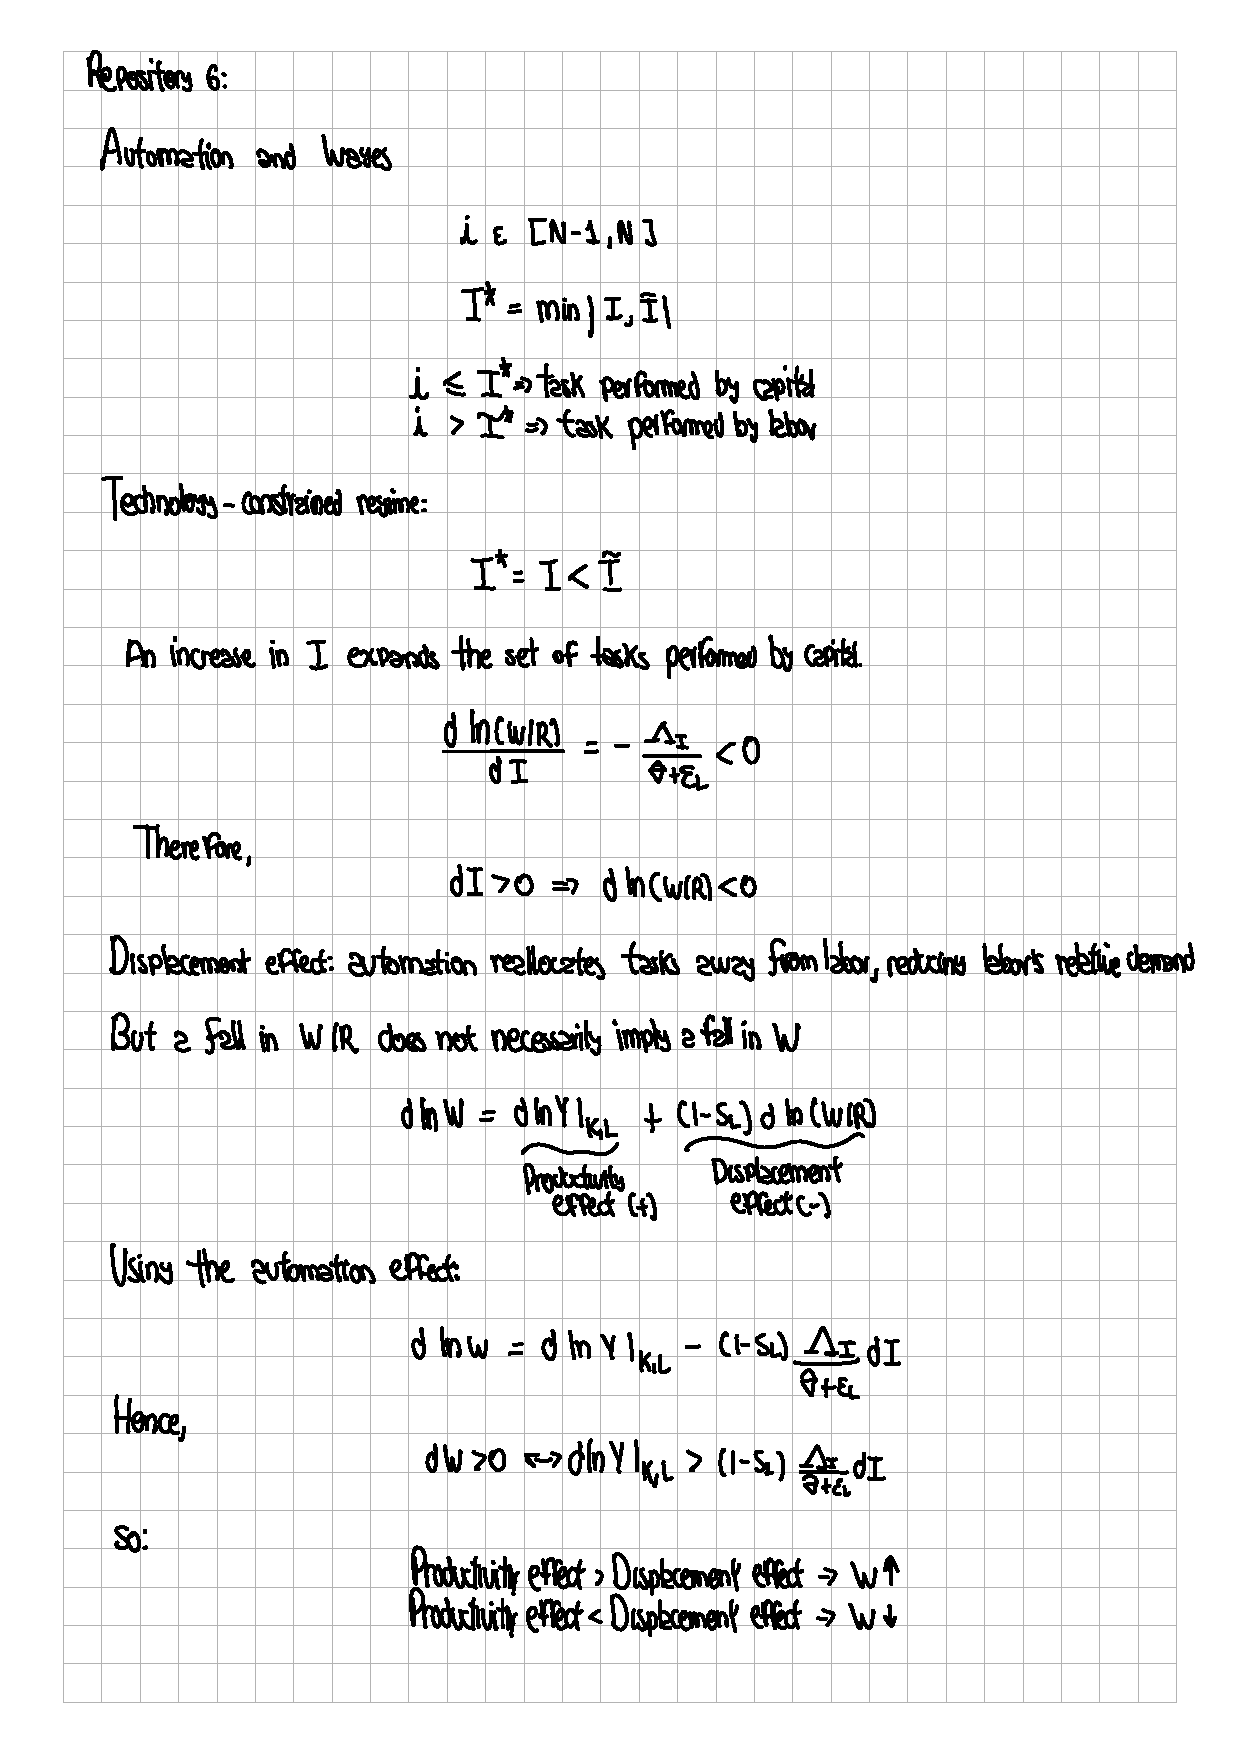
\includegraphics[
      page=1,
      height=0.68\textheight,
      keepaspectratio
    ]{hand/prop3-automation-wages.pdf}
  }{
    Missing hand derivation.
  }

  \vspace{0.3em}

  \small
  \textbf{Question I checked:}
  Does
  $
    \frac{d\ln(W/R)}{dI}<0
  $
  imply
  $
    \frac{dW}{dI}<0
  $?
  \quad
  \textbf{No: the first is a relative-price result.}

\end{frame}

% ============================================================
% 13
% ============================================================

\begin{frame}{13 \textperiodcentered{} Where I did not believe the AI: hand check II}

  \centering

  \IfFileExists{hand/prop3-automation-wages.pdf}{
    \includegraphics[
      page=2,
      height=0.68\textheight,
      keepaspectratio
    ]{hand/prop3-automation-wages.pdf}
  }{
    Missing hand derivation.
  }

  \vspace{0.3em}

  \small
  \textbf{Verdict:}
  $
    d\ln W
    =
    \text{productivity effect}
    -
    \text{displacement effect}.
  $

  The sign of $dW$ is ambiguous even though
  $W/R$, the labor share, and employment fall.

\end{frame}

% ============================================================
% 14
% ============================================================

\begin{frame}{14 \textperiodcentered{} Lean: paper claim before code}

  \textbf{Source-facing mathematical core of Proposition 3}

  \[
    \text{cost saving}>0
    \quad\Longrightarrow\quad
    \text{productivity contribution}>0.
  \]

  In the reduced-form formalization,

  \[
    \texttt{productivityContribution}
    =
    \texttt{scale}
    \left(
      \texttt{expensive}-\texttt{cheap}
    \right).
  \]

  Hence the checked sign claim is

  \[
    \texttt{scale}>0,
    \qquad
    \texttt{cheap}<\texttt{expensive}
  \]

  \[
    \Longrightarrow
    \quad
    \texttt{productivityContribution}>0.
  \]

  The wage and rental decompositions are represented separately
  as exact algebraic identities.

\end{frame}

% ============================================================
% 15
% ============================================================

\begin{frame}[fragile]{15 \textperiodcentered{} Lean: statement and proof fragment}

\begin{lstlisting}
theorem productivityContribution_pos
    {scale expensive cheap : ℝ}
    (hscale : 0 < scale)
    (hcost : cheap < expensive) :
    0 < productivityContribution scale expensive cheap := by
  exact mul_pos hscale (sub_pos.mpr hcost)
\end{lstlisting}

\vspace{0.3em}

\begin{lstlisting}
theorem proposition3_productivity_factor_price_core :
    proposition3_productivity_factor_price_coreSpec := by
  intro scale expensive cheap productivity laborShare
    relativePriceChange hscale hcost
  exact ⟨
    productivityContribution_pos hscale hcost,
    wageChangeDecomposition_eq
      productivity laborShare relativePriceChange,
    rentalChangeDecomposition_eq
      productivity laborShare relativePriceChange
  ⟩
\end{lstlisting}

\end{frame}

% ============================================================
% 16
% ============================================================

\begin{frame}{16 \textperiodcentered{} What Lean verifies -- and what it does not}

  \begin{itemize}\small

    \item \textbf{Objects:}
    real-valued reduced-form quantities for scale, costs,
    productivity, labor share, and relative-price change.

    \item \textbf{Nontrivial proof step:}
    \texttt{sub\_pos.mpr hcost} proves
    \[
      \texttt{expensive}-\texttt{cheap}>0,
    \]
    and \texttt{mul\_pos} combines it with positive scale.

    \item \textbf{Exact identities:}
    the wage and rental decompositions close by definitional
    equality in the underlying model file.

    \item \textbf{Boundary:}
    Lean does \emph{not} derive these reduced-form quantities
    from the full continuum-task equilibrium or prove the full
    $K\gtrless\widetilde K$ threshold.

  \end{itemize}

  \medskip

  \textbf{Final check}

  \[
    \texttt{Build completed successfully (832 jobs), exit\_code=0.}
  \]

\end{frame}

% ============================================================
% 17
% ============================================================

\begin{frame}{17 \textperiodcentered{} What the formalization exercise taught me}

  \begin{itemize}\small

    \item A successful build is only meaningful relative to the
    statement that was encoded.

    \item The paper's economic content lives in the bridge from
    the task economy to the reduced-form comparative statics.

    \item Lean is strongest here at exposing exactly which sign
    conditions are assumed and which conclusions follow algebraically.

    \item The main remaining formalization challenge is therefore
    \textbf{economic}: formalize the continuum task allocation and
    derive Proposition 3 rather than starting from its reduced form.

  \end{itemize}

\end{frame}

% ============================================================
% 18
% ============================================================

\begin{frame}{18 \textperiodcentered{} Takeaways}

  \begin{enumerate}\small

    \item Automation is not just factor-augmenting technical change:
    it reallocates tasks from labor to capital.

    \item In the technology-constrained regime, automation lowers
    $W/R$, the labor share, and employment.

    \item The real wage is ambiguous because productivity and
    displacement push in opposite directions.

    \item New tasks generate reinstatement and push labor demand
    in the opposite direction.

    \item The long-run question is therefore not simply
    ``man or machine?'' but which margin advances faster:
    automation or new labor-intensive tasks.

  \end{enumerate}

  \medskip

  \begin{center}
    \small
    \texttt{github.com/carlosgomezp28/ai-06-restrepo}
  \end{center}

\end{frame}

\end{document}
EOF